\chapter{Sistemi di equazioni non lineari}

Fino ad ora siamo sempre stati abituati a problemi analitici dove la soluzione a un problema era data da un'equazione, o al più un piccolo sistema di equazioni non lineari. Tuttavia nella realtà sono molti i casi dove la soluzione viene trovata risolvendo complessi sistemi di equazioni non lineari, che non sempre possono essere svolti a mano. Da qui, la nascita di alcuni metodi di calcolo numerico che aiutano nella risoluzione di tali sistemi. Prima di illustrare questi metodi, ci soffermeremo brevemente su cos'è un'equazione non lineare:

\begin{definition}{Equazione non lineare}
    Un'\textbf{equazione non lineare} è un'equazione avente la forma
    \[ f(x) \eq 0 \]

    Chiamamo \textbf{soluzione} $\xi$ (o alternativamente \textbf{radici dell'equazione} o \textbf{zeri della funzione} $f$) di un'equazione non lineare quel valore tale che
    \[ f(\xi) \eq 0 \]
\end{definition}

All'interno di questo capitolo ci limiteremo prevalentemente al caso di radici reali. Per applicare un metodo su una funzione tuttavia, ci serve prima sapere le seguenti tre informazioni:
\begin{itemize}
    \item [1)] \textbf{quante} sono le radici (in questo caso, reali);
    \item [2)] \textbf{dove} si trovano, approssimativamente, le radici;
    \item [3)] se sono presenti delle \textbf{simmetrie} nella funzione.
\end{itemize}

Ci sono vari metodi per trovare queste informazioni: si può procedere allo \textbf{studio analitico}, alla \textbf{tabulazione} o all'analisi del \textbf{grafico} della funzione stessa. Procederemo ad illustrare tutti e tre i metodi su un'equazione di esempio:

\begin{example}
    Si consideri la seguente funzione $f(\lambda)$, che modella il tasso di crescita di una popolazione:
    \[ f(\lambda) \eq e^{\lambda} + \frac{0,435}{\lambda} (e^{\lambda} - 1) - 1,564 \eq 0 \]

    Procediamo a considerare lo \textbf{studio analitico} di questa funzione: notiamo che la funzione risulta definita e continua in $\mathbb{R} / \{0\}$, e studiando il semiasse positivo (non ha senso controllare il semiasse negativo, poiché quest'equazione modella la crescita della popolazione) notiamo che:
    \[ \lim_{\lambda \to 0} f(\lambda) < 0 \quad\quad \text{e} \quad\quad \lim_{\lambda \to +\infty} f(\lambda) \eq +\infty \]

    Calcolando la derivata prima, otteniamo invece la seguente funzione:
    \[ f'(\lambda) \eq e^{\lambda} + \left( 1 + 0,435 \frac{\lambda - 1}{\lambda^2} \right) + \frac{0,435}{\lambda^2} > 0 \]

    Notiamo infatti che il comportamento della funzione è positivo oltre lo 0: questo significa che la funzione $f(\lambda)$ è monotona crescente. Possiamo dunque concludere che, nel semiasse positivo, sia presente un unico zero $\xi$.
    \nwl
    Per il metodo della \textbf{tabulazione}, si considerano i valori ottenuti dalla funzione in corrispondenza di valori equidistanti di $\lambda$, e si osserva dunque il segno dei valori ottenuti. Ad esempio:
    \begin{center}
        \begin{tabular}{c|c}
            $\lambda$ & $f(\lambda)$ \\
            \hline
            $0,10$ & $-0,001335588295285$ \\
            $0,12$ & $0,025672938554613$ \\
            $0,14$ & $0,053195959592184$ \\
            $0,16$ & $0,081243551500795$ \\
            $0,18$ & $0,109825990666185$ \\
            $0,20$ & $0,138953757158539$ \\
        \end{tabular}
    \end{center}

    Come possiamo notare, abbiamo un cambio di segno tra $\lambda \eq 0,10$ e $\lambda \eq 0,12$: questo vuol dire che la radice della funzione si trova nell'intervallo $[0,10, \; 0,12]$. Possiamo anche osservare la radice usando un grafico della funzione:
    \begin{center}
        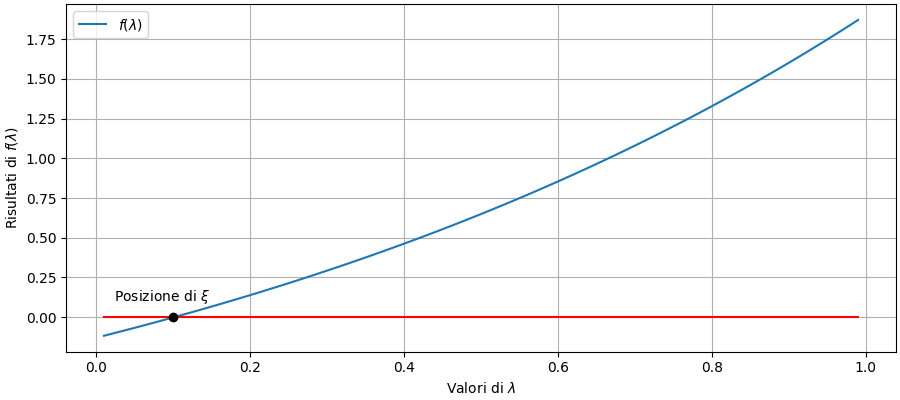
\includegraphics[width=\linewidth]{assets/image-002.png}
    \end{center}
\end{example}

Come abbiamo potuto notare dall'esempio, grazie ai tre metodi possiamo trovare una posizione approssimativa delle varie radici di una funzione. Ma come mai ci interessa tanto sapere la posizione di dove la funzione cambia segno? Perché grazie al \textbf{teorema di Bolzano}, questo ci permette di localizzare una radice.

\begin{theorem}{Teorema di Bolzano}
    Dato un \textbf{intervallo} $[a, \; b]$ e una \textbf{funzione} $f(x)$ \textbf{continua}, se $f(a)$ ha \textbf{segno discorde} rispetto a $f(b)$ (quindi, se $f(a) \cdot f(b) < 0$), allora $f(x)$ \textbf{interseca almeno una volta} l'asse delle $x$
\end{theorem}

È importante tuttavia sapere anche restringere l'intervallo di osservazione delle radici. Supponiamo di avere in esame la funzione
\[ p(x) \eq x^4 + 2x^3 + 7x^2 - 11 \eq 0 \]

mostriamo qui due grafici della funzione, in intervalli diversi:
\begin{center}
    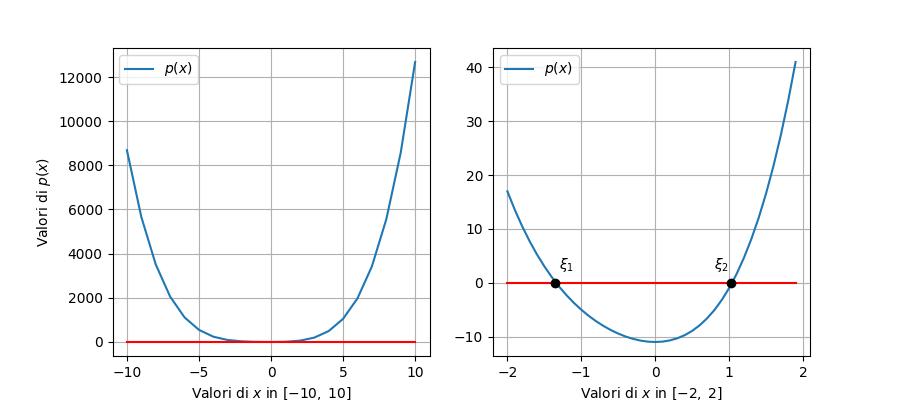
\includegraphics[width=\linewidth]{assets/image-003.png}
\end{center}

Notiamo come, in base all'intervallo, è più semplice notare la posizione delle radici. Infatti, $p(x)$ ha 4 radici, di cui due reali e due complesse coniugate.

\section{Metodo di bisezione (o dicotomico)}

Tra i vari metodi utilizzabili per trovare le radici in una funzione, il più semplice e immediato da utilizzare è il \textbf{metodo di bisezione}, o \textbf{metodo dicotomico}. Questo metodo permette, una volta individuato un intervallo di separazione in cui si trova una \textbf{singola radice}, di costruire una successione $\{ x_k \}$ di approssimazioni di $\xi$. Per applicare dunque questo metodo vanno rispettate due condizioni, dette \textbf{ipotesi di applicabilità}:
\begin{itemize}
    \item è stato individuato un intervallo $I \eq [a, \; b]$, all'interno del quale è presente \textbf{un'unica radice} $\xi$;
    \item la funzione $f$ in esame deve essere \textbf{continua in} $I$ (formalmente, $f \in C^0 [a, \; b]$, dove $C^0$ è l'insieme di funzioni continue);
    \item i due estremi $a$ e $b$ devono avere \textbf{segno discorde} (dunque $f(a) \cdot f(b) < 0$).
\end{itemize}

In sintesi, il teorema di Bolzano deve essere rispettato all'interno del nostro intervallo $I$; il metodo di bisezione infatti usa estensivamente il suddetto teorema. Passiamo dunque ad esaminare l'algoritmo del metodo di bisezione:

\begin{algorithm}[H]
    \caption{Metodo di bisezione (o dicotomico)}
    \KwIng{L'intervallo $[a, b]$, la funzione $f(x)$ e la tolleranza}
    $a \gets a_0, \; b \gets b_0$\;
    $\xi_{\text{seq}} \gets \{\}$ \tcp*{$\xi_{\text{seq}}$ è una sequenza vuota}
    \For{$k$ in $1, \; 2, \; 3, \; ...$}{
        $x_k \gets \frac{a + b}{2}$\;
        $d \gets |x_k - x_{k - 1}|$\;
        \BlankLine
        Aggiungere $x_k$ a $\xi_{\text{seq}}$\;
        \BlankLine
        \tcp{Se si trova la radice oppure viene raggiunta la tolleranza, l'algoritmo si ferma}
        \If{$(f(x_k) = 0)$ \textbf{or} $(d < \text{tol})$}{
            \textbf{return} $\xi_{\text{seq}}$
        }
        \BlankLine
        \tcp{In base all'intervallo che contiene la radice, ripetere l'algoritmo con l'intervallo aggiornato}
        \If{$f(a) \cdot f(x_k) < 0$}{
            $a \gets a, \; b \gets x_k$
        }
        \BlankLine
        \If{$f(x_k) \cdot f(b) < 0$}{
            $a \gets x_k, \; b \gets b$
        }
    }
\end{algorithm}

\nwl
Per il metodo di bisezione, l'idea è che dato un intervallo $I = [a, \; b]$, \textbf{dividendo} $I$ sempre \textbf{in sotto-intervalli} più contenuti, riusciremmo eventualmente ad ottenere un intervallo più piccolo all'interno del quale troveremmo la nostra radice $\xi$. Ogni sotto-intervallo è costituito da una delle due metà di $I$. Per sapere quale sotto-intervallo contiene $\xi$, basta applicare il teorema di Bolzano. L'algoritmo è semplice, e genera una successione di tutte le approssimazioni di $\xi$, denominata $\{x_k\}$ (o, nell'algoritmo, $\xi_{\text{seq}}$). La precisione del metodo di bisezione è ottenibile calcolando il relativo \textbf{errore di troncamento}.

\begin{definition}{Errore di troncamento}
    L'\textbf{errore di troncamento} è l'errore commesso \textbf{approssimando} la radice $\xi$ con il $k$-esimo elemento della successione creata tramite l'algoritmo del metodo di bisezione
    \[ e_k \eq \xi - x_k \]
\end{definition}

Ma l'algoritmo \textbf{può convergere}? Intuitivamente, convergerà verso $\xi$ solo se l'errore si dovesse ridurre a 0. Formalmente, possiamo esprimere questa relazione come
\[ \lim_{k \to \infty} x_k \eq \xi \quad \Longleftrightarrow \quad \lim_{k \to \infty} |e_k| \eq 0 \]

Possiamo però esprimere $e_k$ anche in altri termini. Per il metodo di bisezione, noi sappiamo che alla $k$-esima iterazione, $\xi$ sarà presente solo in $[a_{k - 1}, \; x_k]$ o in $[x_k, \; b_{k - 1}]$.

\begin{center}
    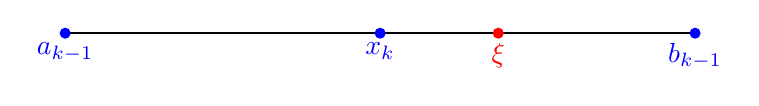
\begin{tikzpicture}
        \draw[black, thick] (0, 0) -- (8, 0);
        \fill[blue] (0, 0) circle (2pt) node [below] {$a_{k - 1}$};
        \fill[blue] (4, 0) circle (2pt) node [below] {$x_k$};
        \fill[blue] (8, 0) circle (2pt) node [below] {$b_{k - 1}$};
        \fill[red] (5.5, 0) circle (2pt) node [below] {$\xi$};
    \end{tikzpicture}
\end{center}

Dunque, data una generica iterazione $x_k$, l'errore di troncamento alla suddetta sarà uguale a
\[ |e_k| < \frac{b_{k - 1} - a_{k - 1}}{2} \]

Ora, siccome l'intervallo $[a_{k - 1}, \; b_{k - 1}]$ ha ampiezza pari alla metà dell'intervallo all'iterazione precedente (dunque $[a_{k - 2}, \; b_{k - 2}]$), possiamo costruire anche una formula generica dell'errore per qualsiasi iterazione $k$:
\[ |e_k| < \frac{b_{k - 1} - a_{k - 1}}{2} = \frac{b_{k - 2} - a_{k - 2}}{2^2} \eq \; ... \; \eq \frac{b - a}{2^k} \]

Dunque, anche il limite di prima può essere riscritto come
\[ 0 \leq \lim_{k \to \infty} |e_k| < \lim_{k \to \infty} \frac{b - a}{2^k} = 0 \]

\subsection{Ordine di corvengenza e criteri di arresto}

Abbiamo visto che il metodo di bisezione converge, ma è anche importante che converga in tempi rapidi. Come possiamo determinare la "velocità" di convergenza? Questo viene determinato in base a un valore chiamato \textbf{ordine di convergenza} $p$.

\begin{definition}{Ordine e Fattore di Convergenza}
    Sia $\{ x_k \}$ una successione di approssimazioni \textbf{convergente} a $\xi$. Si dice che la successione ha un \textbf{ordine di convergenza} $p$ e un \textbf{fattore di convergenza} $C$ se esistono due numeri reali $p \geq 1$ e $C > 0$ tali che
    \[ \lim_{k \to \infty} \frac{|e_{k + 1}|}{|e_k|^p} \eq C \]

    Se $p \eq 1$, si dice che la convergenza è \textbf{lineare}, se $p \eq 2$, si dice invece che la convergenza è \textbf{quadratica}.
\end{definition}

Applicando la definizione di ordine e fattore di convergenza al metodo di bisezione, otteniamo che, per $k \to \infty$, si ha:
\[ \frac{|e_{k + 1}|}{|e_k|^p} \eq \frac{\frac{b - a}{2^{k + 1}}}{\frac{b - a}{2^k}} \eq \frac{2^k}{2^{k + 1}} \eq \frac{2^k}{2^k} \cdot \frac{1}{2} \eq \frac{1}{2} \]

Cosa ci dice il risultato appena ottenuto? Che, \textbf{supponendo una convergenza lineare}, otteniamo un \textbf{fattore di convergenza} di $\nicefrac{1}{2}$. Questo ci dice che la convergenza è in realtà \textbf{lenta}: ad ogni step dell'algoritmo riusciamo a dimezzare l'errore, e guadagnamo una cifra binaria per meglio esprimere il nostro risultato. Siccome $2^{-4} < 10^{-1} < 2^{-3}$, allora ogni 3 o 4 iterazioni si riesce a guadagnare una cifra decimale.
\nwl
Tuttavia, a causa degli errori di arrotondamento e troncamento da parte del computer, è praticamente impossibile che si riesca a raggiungere $f(x_k) \eq 0$. Dunque, quando dovremmo interrompere i calcoli? Possiamo definire dei \textbf{criteri di arresto a posteriori}, ovverosia
\[ \begin{cases}
|e_k| \simeq |x_k - x_{k - 1}| < \epsilon & \text{Se l'errore diventa minore di una tolleranza } \epsilon ... \\
|f(x_k)| < \epsilon & \text{...o se la funzione ritorna numeri minori della tolleranza } \epsilon
\end{cases} \]

Nel caso dell'algoritmo di bisezione, è stato scelto in precedenza di usare il primo criterio, ma potevano essere usati entrambi i criteri. Possiamo anche calcolare \textbf{a priori} una stima di quante iterazioni $K$ avremo bisogno prima di ottenere un errore minore di $\epsilon_{\text{min}}$. Per farlo, ci avvaliamo della formula dell'errore di troncamento:
\[ |e_k| < \frac{b - a}{2^k} < \epsilon_{\text{min}} \quad \Longrightarrow \quad K > \frac{\log(b - a) - \log(\epsilon_{\text{min}})}{\log(2)} \]

$K$ dovrà essere arrotondato all'intero più vicino, in quanto deve essere un intero positivo.

\section{Metodo di Newton-Raphson}

Forse uno dei metodi più utilizzati quando si parla di equazioni non lineari, il \textbf{metodo di Newton-Raphson} (o metodo delle tangenti) è un metodo molto usato, grazie alla sua convergenza più immediata rispetto al metodo di bisezione. Questo metodo prevede di approssimare una funzione $f(x)$ in un intorno $I$, all'interno del quale si deve trovare una e una sola radice $\xi$, grazie alle sue \textbf{tangenti} in vari punti, le quali vengono calcolate grazie ad uno \textbf{sviluppo in serie di Taylor}.
\nwl
Partendo da un'approssimazione iniziale della radice, che chiameremo $x_0$, è possibile costruire la tangente $t_0$ alla funzione nel punto di intersezione tra $x = x_0$ e la funzione stessa (quindi, nel punto $(x_0, \; f(x_0))$). Per costruire la tangente, viene utilizzato lo sviluppo in serie di Taylor (\textbf{fino al primo ordine}), che tramite il calcolo della derivata prima permette di trovare l'equazione di $t_0$:
\[ t_0 \eq f(x_0) + f'(x_0) \cdot (x - x_0) \]

Calcolata la tangente, si procede recuperando il punto di intersezione tra $t_0$ e l'asse delle $x$; tale punto viene chiamato $x_1$. Una volta ottenuto $x_1$, il procedimento ricomincia da capo: si trova dunque il punto di intersezione $(x_1, \; f(x_1))$, si calcola la tangente $t_1$ nel punto appena trovato (quindi $t_1 \eq f(x_1) + f'(x_1) \cdot (x - x_1)$) e si ottiene un nuovo punto, chiamato $x_2$. Il procedimento continua finché non si raggiunge o la radice o un criterio d'arresto.
\nwl
Generalmente, ad ogni iterazione $k \eq 1, \; 2, \; ...$ del metodo, la nuova approssimazione della radice $x_k$ è data dall'intersezione tra la tangente $t_k$ a $f(x)$ nel punto $(x_{k - 1}, \; f(x_{k - 1}))$ e l'asse delle $x$:
\[ t_{k} \eq f(x_k) + f'(x_k) \cdot (x - x_k) \quad \Longrightarrow \quad \text{si vuole risolvere} \quad f(x_k) + f'(x_k) \cdot (x - x_k) \eq 0 \]

\begin{center}
    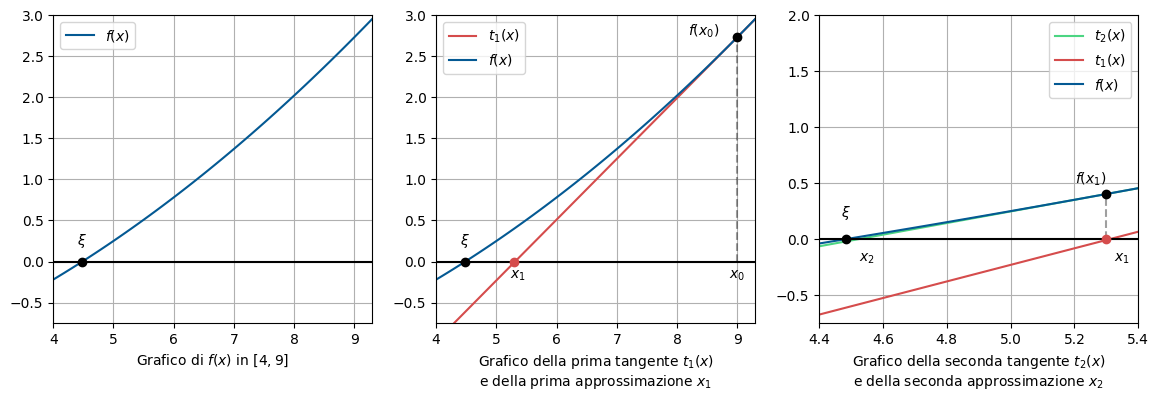
\includegraphics[trim=0 0 0 0, clip=false, width=\textwidth]{assets/image-004.png}
\end{center}

Possiamo tuttavia rifattorizzare l'espressione, così da renderla in funzione dell'approssimazione in un'iterazione $k$:
\begin{align*}
    f(x_{k - 1}) + f'(x_{k - 1}) \cdot (\underbrace{x}_{\text{diventa } x_k} - x_{k - 1}) &\eq 0 \\
    f(x_{k - 1}) + x_k \cdot f'(x_{k - 1}) - x_{k - 1} \cdot f'(x_{k - 1}) &\eq 0 \\
    -x_k \cdot f'(x_{k - 1}) &\eq f(x_{k - 1}) - x_{k - 1} \cdot f'(x_{k - 1}) \\
    -x_k &\eq \frac{f(x_{k - 1})}{f'(x_{k - 1})} - x_{k - 1} \cdot \frac{f'(x_{k - 1})}{f'(x_{k - 1})} \\
    x_k &\eq x_{k - 1} - \frac{f(x_{k - 1})}{f'(x_{k - 1})}
\end{align*}

L'algoritmo, dal punto di vista matematico, diventa dunque il seguente:
\[ \begin{cases}
    x_0 & \text{viene dato come input} \\
    x_k \eq x_{k - 1} - \frac{f(x_{k - 1})}{f'(x_{k - 1})} & \text{per } k \eq 1, \; 2, \; ...
\end{cases} \]
\nwl
Viene qui mostrato l'algoritmo del metodo:
\nwl
\begin{algorithm}[H]
    \caption{Metodo di Newton-Raphson (o delle tangenti)}
    \KwIng{La funzione $f(x)$, un'approssimazione iniziale $x_0$ e la tolleranza}
    $x_k \gets x_0$\;
    $\xi_{\text{seq}} \gets \{\}$\;
    \BlankLine
    \tcp{Finché $x_k$ non è uguale a $\xi$ oppure finché non si raggiunge la tolleranza...}
    \While {$(f(x_k) \neq 0)$ \textbf{or} $(x_k > \text{tol})$}{
        \tcp{...calcola la nuova approssimazione di $\xi$}
        $x_{k + 1} \gets x_k - \frac{f(x_k)}{f'(x_k)}$\;
        Aggiungere $x_{k + 1}$ a $\xi_{\text{seq}}$\;
        $x_k \gets x_{k + 1}$\;
    }
    \BlankLine
    \textbf{return} $x_k$, $\xi_{\text{seq}}$
\end{algorithm}

\nwl
Procediamo a mostrare questo metodo attraverso un esempio:

\begin{example}
    Calcolare la radice quadrata di un numero $a$ è equivalente al trovare gli zeri della funzione
    \[ f(x) \eq x^2 - a \]

    Per trovare gli zeri, vogliamo ricorrere al metodo di Newton-Raphson. Modellando l'algoritmo definito in precedenza, otteniamo la seguente equazione:
    \[ \begin{cases}
        x_0 & \text{dato come input} \\
        x_k \eq x_{k - 1} - \frac{x^2_{k - 1} - a}{2x_{k - 1}} & \text{per } k \eq 1, \; 2, \; ...
    \end{cases} \]

    Possiamo ulteriormente semplificare l'algoritmo, raggiungendo dunque la seguente equazione:
    \[ \begin{cases}
        x_0 & \text{dato come input} \\
        x_k \eq \frac{1}{2} \cdot \left( x_{k - 1} \right) & \text{per } k \eq 1, \; 2, \; ...
    \end{cases} \]
\end{example}

Similmente al metodo di bisezione, possiamo definire se l'algoritmo di Newton-Raphson convergerà, definendo dunque le sue condizioni di convergenza.

\begin{theorem}{Convergenza del metodo di Newton-Raphson: esistenza di $J$}
    Data una funzione $f(x)$, se:
    \begin{itemize}
        \item è stato separato un intervallo $I \eq [a, \; b]$ dove c'è una \textbf{singola} radice $\xi$;
        \item $f, \; f', \; f''$ sono continue in $I$, tale che $f \in C^2 [a, \; b]$;
        \item $f'(x) \neq 0$ per $x \in [a, \; b]$;
    \end{itemize}

    allora esiste un intorno $J \subseteq I$ di $\xi$ tale che, se $x_0 \in J$, allora la successione delle approssimazioni convergerà a $\xi$.

    \begin{center}
        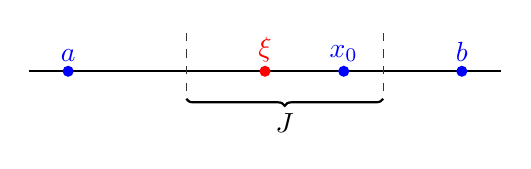
\begin{tikzpicture}
            \draw[black, thick] (0, 0) -- (6, 0);
            \fill[blue] (0.5, 0) circle (2pt) node[anchor=south] {$a$};
            \fill[blue] (5.5, 0) circle (2pt) node[anchor=south] {$b$};
            \fill[blue] (4, 0) circle (2pt) node[anchor=south] {$x_0$};
            \fill[red] (3, 0) circle (2pt) node[anchor=south] {$\xi$};
            \draw[thick, decoration={brace, mirror, raise=1mm}, decorate] (2, -0.25) -- (4.5, -0.25) node [pos=0.5, anchor=north, yshift=-1.5mm] {$J$};
            \draw[black!80, dashed] (2, -0.25) -- (2, 0.5);
            \draw[black!80, dashed] (4.5, -0.25) -- (4.5, 0.5);
        \end{tikzpicture}
    \end{center}
\end{theorem}

Il precedente teorema non stabilisce che il metodo convergerà, ma che piuttosto esiste un intervallo $J$, ristretto rispetto a $I$, nel quale troveremo la nostra radice $\xi$.

\subsection{Ordine di convergenza}

Per valutare l'ordine di convergenza del metodo, usiamo la stessa formula per trovare $C$, ovverosia
\[ C \eq \lim_{k \to \infty} \frac{|e_{k + 1}|}{|e_k|^p} \]

Sappiamo che l'errore di troncamento all'interazione $k + 1$ è uguale alla differenza tra la radice e l'approssimazione ottenuta in quello step: dunque, possiamo sviluppare il calcolo come segue:
\[ e_{k + 1} \eq \xi - x_{k + 1} \eq \left(\xi - \frac{f(\xi)}{f'(\xi)}\right) - \left(x_k - \frac{f(x_k)}{f'(x_k)}\right) \eq (\xi - x_k) - \left(\frac{f(\xi)}{f'(\xi)} - \frac{f(x_k)}{f'(x_k)}\right) \]

Per determinare $f(x_k)$ è sufficiente sviluppare i primi tre termini dello sviluppo in serie di Taylor attorno a $\xi$, dunque:
\[ f(x_k) \eq f(\xi) + f'(\xi) \cdot \underbrace{(x_k - \xi)}_{-e_k} + \frac{1}{2} f''(\xi) \cdot (x_k - \xi)^2 + \; ... \]

Supponendo che $x_k$ sia molto vicino a $\xi$, possiamo assumere con condifenza che le derivate di $f$ in $x_k$ e $\xi$ assumano valori simili ($f'(x_k) \simeq f'(\xi)$). Possiamo ora sostituire i valori di $f(x_k)$ e $f'(x_k)$ nell'espressione di $e_{k + 1}$, ottenendo:
\[ |e_{k + 1}| \simeq \left\lvert e_k - \frac{f(\xi) - \overbrace{f(\xi) + f'(\xi) \cdot e_k - \frac{1}{2} f''(\xi) \cdot e_k^2}^{f(x_k)}}{f'(\xi)} \right\rvert \eq \left\lvert \frac{\frac{1}{2} f''(\xi) \cdot e_k^2}{f'(\xi)} \right\rvert \]

Ottenuta questa forma, possiamo sostituire $e_{k + 1}$ nel limite che definisce $C$ con ciò che abbiamo appena trovato. Otteniamo dunque la seguente forma:
\[ \lim_{k \to \infty} \frac{|e_{k + 1}|}{|e_k|^2} \eq \frac{1}{2} \cdot \left\lvert \frac{f''(\xi)}{f'(\xi)} \right\rvert \; \Longrightarrow \; p \geq 2 \]

Dunque, se $f(x) \in C^3 [a, \; b]$, avremo una convergenza almeno quadratica. Nella precedente espressione, abbiamo usato nel limite $p \eq 2$: questo valore potrebbe anche essere uguale a 3 in alcuni casi, ma verrà visto in futuro come questo può cambiare.

\subsection{Efficienza computazionale}

Quando va scelto un metodo numerico, non solo si vuole scegliere un metodo che sia preciso, ma che porti anche alla soluzione in tempi rapidi. A livello informatico questo viene calcolato tramite la notazione "\textit{O grande}" $O(\cdot)$. Per ora, ci interesseremo dell'\textbf{efficienza} di un nostro metodo, che ci darà una valutazione oggettiva di quanto bene il metodo performi.

\begin{definition}{Efficienza computazionale}
    Definiamo come \textbf{efficienza computazionale} $E$, dato un \textbf{ordine di convergenza} $p$ e un numero di \textbf{valutazioni funzionali} $r$ (ovverosia il numero di calcolo di funzioni o derivate) richieste ad ogni passo, il valore dato dalla seguente formula:
    \[ E \eq p^{\frac{1}{r}} \]
\end{definition}

Applicando il concetto di efficienza computazionale sia al metodo di bisezione che al metodo di Newton-Raphson otteniamo i seguenti risultati:
\begin{itemize}
    \item il metodo di bisezione richiede, ad ogni iterazione, una sola valutazione funzionale, ovverosia solo $f(x_k)$: abbiamo dunque che $r \eq 1$. Supponendo $p \eq 1$, otteniamo che $E$ è uguale a:
    \[ E \eq 1^{\nicefrac{1}{1}} \eq 1 \]
    \item il metodo di Newton-Raphson richiede, per ogni iterazione, due valutazioni funzionali, siccome van calcolati sia $f(x_k)$ che $f'(x_k)$: abbiamo dunque $r \eq 2$. Ponendo $p \eq 2$, il valore di $E$ è uguale a:
    \[ E \eq 2^{\nicefrac{1}{2}} \eq \sqrt{2} \]
\end{itemize}

\subsection{Ottimizzazione tramite estremo di Fourier}

Fino ad ora non abbiamo mai considerato la possibilità che certe ottimizzazioni siano più efficienti di altre, e abbiamo sempre supposto che $x_0$ ci venisse data da qualche entità superiore. Tuttavia esiste un modo per determinare quale approssimazione è più efficace per avere una convergenza più rapida (o, in generale, per avere una convergenza!). Illustreremo l'importanza di una buona ottimizzazione usando il seguente esempio:

\begin{example}
    Vogliamo approssimare la redice $\xi \eq 0$ dell'equazione
    \[ f(x) \eq 4x^3 - 5x \eq 0 \]

    Come intervallo, scegliamo $I \eq [-0.5, \; 0.5]$, e decidiamo di iniziare con $x_0 \eq 0.5$. Già dopo due iterazioni, notiamo che c'è un problema con le tangenti:
    \begin{center}
        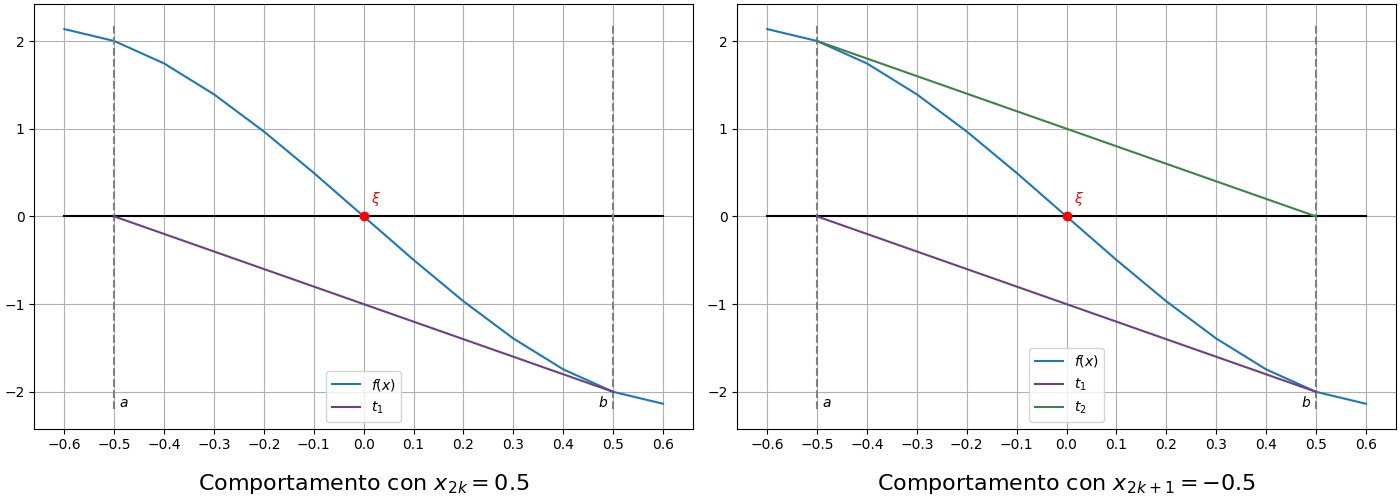
\includegraphics[width=\linewidth]{assets/image-005.png}
    \end{center}

    Come possiamo notare, le tangenti, per ogni iterazione pari di $k$, portano da $x \eq 0.5$ a $x \eq -0.5$, mentre invece le iterazioni dispari ritornano a $x \eq 0.5$: si genera dunque una \textbf{situazione di stallo}. Questa situazione rispetta comunque il criterio di applicabilità del metodo di Newton-Raphson: infatti, la funzione $f(x)$ e la sua derivata $f'(x) \eq 12x^2 - 5$ sono entrambe continue in $C^2 (I)$. La situazione cambia scegliendo altri valori di $x_0$, come ad esempio $x_0 = 0.4$:

    \begin{center}
        \begin{tabular}{|c|c|c|c|}
            \hline
            $k$ & $x_k$ & $|x_k - x_{k - 1}|$ & $\left\lvert f(x_k) \right\rvert$ \\
            \hline\hline
            1 & -0.166233766233766 & 0.566233766233766 & 0.812794238313550 \\
            \hline
            2 & 0.007871908372072 & 0.174105674605839 & 0.039357590668022 \\
            \hline
            3 & -0.000000780593026 & 0.007872688965099 & 0.000000390296513 \\
            \hline
            4 & 0.000000000000000 & 0.000000780593026 & 0.000000000000000 \\
            \hline
        \end{tabular}
    \end{center}
\end{example}

Come abbiamo potuto notare, è possibile che si verifichino episodi di stallo quando selezioniamo $x_0$: in particolare, questo accade quando si scelgono come approssimazioni iniziali dei punti non appartenenti ad un opportuno intorno $J$. Fatta questa analisi, è possibile però scegliere dei punti che non creino queste situazioni? La possibilità c'è, ed è data dall'\textbf{estremo di Fourier}.

\begin{definition}{Estremo di Fourier}
    Data una funzione $f$, \textbf{continua} e \textbf{convessa} in $I = [a, \; b]$, con $f(a) \cdot f(b) < 0$, allora chiamiamo l'\textbf{estremo di Fourier} di $I$ l'estremo verso cui $f$ rivolge la convessità.
    \nwl
    Inoltre, se $\exists \; f''$, allora l'estremo di Fourier assume i seguenti valori:
    \[ \begin{cases}
        a & \text{se } f(a) \cdot f''(a) > 0 \\
        b & \text{se } f(b) \cdot f''(b) > 0
    \end{cases} \]
\end{definition}

Con questo nuovo elemento, possiamo ridefinire i criteri di applicabilità del metodo di Newton-Raphson, in un teorema che sia più comprensivo e che non si limiti al solo intervallo $J$:

\begin{theorem}{Convergenza del metodo di Newton-Raphson}
    Data una funzione $f(x)$, se:
    \begin{itemize}
        \item $f(a) \cdot f(b) < 0$;
        \item $f, \; f', \; f''$ sono continue in $I$, tale che $f \in C^2 [a, \; b]$;
        \item $f'(x) \neq 0$ per $x \in [a, \; b]$;
        \item $f''(x) \neq 0$ per $x \in [a, \; b]$ e $x_0$ è l'estremo di Fourier di $[a, \; b]$;
    \end{itemize}

    allora:
    \begin{itemize}
        \item [1)] \textbf{esiste} un'\textbf{unica radice} $\xi \in [a, \; b]$;
        \item [2)] la successione delle approssimazioni $a_k$ è \textbf{monotona} e \textbf{converge} a $\xi$, dove:
        \[ a_k \eq \left\{ x_k \eq x_{k - 1} - \frac{f(x_{k - 1})}{f'(x_{k - 1})} \right\} \quad\quad \text{per } k \eq 1, \; 2, \; ... \]
        \item [3)] se $f \in C^3 [a, \; b]$, allora la \textbf{convergenza} è \textbf{quadratica}
    \end{itemize}

    \begin{center}
        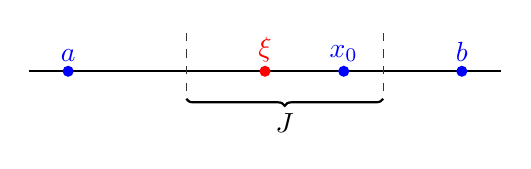
\begin{tikzpicture}
            \draw[black, thick] (0, 0) -- (6, 0);
            \fill[blue] (0.5, 0) circle (2pt) node[anchor=south] {$a$};
            \fill[blue] (5.5, 0) circle (2pt) node[anchor=south] {$b$};
            \fill[blue] (4, 0) circle (2pt) node[anchor=south] {$x_0$};
            \fill[red] (3, 0) circle (2pt) node[anchor=south] {$\xi$};
            \draw[thick, decoration={brace, mirror, raise=1mm}, decorate] (2, -0.25) -- (4.5, -0.25) node [pos=0.5, anchor=north, yshift=-1.5mm] {$J$};
            \draw[black!80, dashed] (2, -0.25) -- (2, 0.5);
            \draw[black!80, dashed] (4.5, -0.25) -- (4.5, 0.5);
        \end{tikzpicture}
    \end{center}
\end{theorem}

\section{Metodo delle secanti}

Nonostante il metodo di Newton-Raphson sia più efficiente del metodo di bisezione, c'è uno step che spesso rallenta il metodo, ovverosia il calcolo della derivata $f'(x)$, che può spesso non essere di facile valutazione (si pensi ai network neurali, che devono calcolare spesso il gradiente dei nodi per la backpropagation). Ci sono dei metodi che vengono usati in alternativa, che approssimano la derivata in alcuni modi:
\begin{itemize}
    \item il \textbf{metodo della tangente fissa}, che approssima, ad ogni iterazione, la derivata $f'(x_n)$ con $f'(x_0)$;
    \item il \textbf{metodo delle secanti con estremi variabili}, che approssima $f'(x_n)$ con un rapporto incrementale;
    \item il \textbf{metodo delle secanti con estremo fisso}, che approssima $f'(x_n)$ con il rapporto incrementale in cui un punto rimane fisso ad ogni iterazione.
\end{itemize}

Ci concentreremo brevemente sul metodo delle secanti con estremi variabili, per dimostrare come questo possa essere usato in alternativa al metodo di Newton-Raphson. Ricordiamo che l'equazione di una secante richiede due punti $x_1$ e $x_2$, quindi per il metodo partiremo da $k \eq 2$ (così da avere un $x_0$ e un $x_1$ iniziale). L'equazione è la seguente:
\[ \frac{x - x_1}{x_2 - x_1} \eq \frac{y - y_1}{y_2 - y_1} \]

Per il metodo delle secanti, ad ogni iterazione $k \eq 2, \; 3, \; ...$, calcoliamo una nuova approssimazione $x_k$, che è data dall'intersezione tra la retta $s_{k - 1}$ e l'asse $y \eq 0$. La retta $s_{k - 1}$ è la secante di $f(x)$ nei punti $(x_{k - 2}, \; f(x_{k - 2}))$ e $(x_{k - 1}, f(x_{k - 1}))$.

Matematicamente, l'algoritmo è formulabile come segue:
\[ \begin{cases}
    x_0, \; x_1 & \text{vengono dati come input} \\
    x_k \eq x_{k - 1} - f(x_{k - 1}) \cdot \frac{x_{k - 1} - x_{k - 2}}{f(x_{k - 1}) - f(x_{k - 2})} & \text{per } k \geq 2
\end{cases} \]

Invece, formalmente l'algoritmo è il seguente:
\nwl
\begin{algorithm}[H]
    \caption{Metodo delle secanti con estremo variabile}
    \KwIng{Due approssimazioni $x_0$ e $x_1$, la funzione $f(x)$ e la tolleranza}
    $x_k \gets \texttt{NULL}$\;
    \tcp{$\xi_{\text{seq}}$ è una sequenza vuota}
    $\xi_{\text{seq}} \gets \{\}$\;
    \While {$(f(x_k) \neq 0)$ \textbf{or} $(x_k > \text{tol})$}{
        \tcp{...calcola la nuova approssimazione di $\xi$}
        $x_{k + 1} \gets x_k - f(x_k) \cdot \frac{x_k - x_{k - 1}}{f(x_k) - f(x_{k - 1})}$\;
        Aggiungere $x_{k + 1}$ a $\xi_{\text{seq}}$\;
        $x_k \gets x_{k + 1}$\;
    }
    \BlankLine
    \textbf{return} $x_k$, $\xi_{\text{seq}}$
\end{algorithm}
\nwl
I vantaggi del metodo delle secanti sono i seguenti:
\begin{itemize}
    \item il metodo è utile quando non si conosce la derivata di $f(x)$, o quando $f(x)$ è nota solo in alcuni punti;
    \item ad ogni passo è richiesta solo una valutazione funzionale.
\end{itemize}

Tuttavia, per poter usare questo metodo necessitiamo di due approssimazioni iniziali $x_0$ e $x_1$, e queste devono essere abbastanza accurate.

\begin{theorem}{Convergenza del metodo delle secanti}
    Data una funzione $f(x)$, se:
    \begin{itemize}
        \item è stato separato un intervallo $I \eq [a, \; b]$ \textbf{simmetrico} intorno alla radice $\xi$;
        \item $f$, $f'$ e $f''$ sono continue in $I \; : \; f \in C^2 [a, \; b]$;
        \item $f'(x) \neq 0$ per $x \in [a, \; b]$;
    \end{itemize}
    allora esiste un intorno $J \subseteq I$ di $\xi$ tale che, se $x_0, x_1 \in J$, allora la successione di approssimazioni (chiamata nell'algoritmo $\xi_{\text{seq}}$), \textbf{converge} a $\xi$ con \textbf{convergenza lineare}, ovverosia $1 < p < 2$.
    \nwl
    Inoltre, se $f''(x) \neq 0$, allora possiamo approssimare l'errore allo step $k + 1$ come segue:
    \[ e_{k + 1} \simeq C_N^{\frac{p}{p + 1}} \cdot e_k^p \]

    dove $p \eq \frac{1 + \sqrt{5}}{2}$ e $C_N$ è la costante asintotica del metodo di Newton-Raphson:
    \[ C_N \eq \frac{f''(\xi)}{2f'(\xi)} \]
\end{theorem}

\section{Metodi iterativi a un punto (o del punto unito)}

Fino ad ora abbiamo visto vari metodi numerici che ci hanno permesso di approssimare le radici, ed ognuno di questi utilizzava dei costrutti matematici come le tangenti o le secanti. Un altro tipo di metodi che possono essere usati per approssimare le radici sono i \textbf{metodi iterativi a un punto}, o \textbf{metodi iterativi del punto unito}, e questi metodi sono utilizzati perché richiedono soltanto un singolo valore iniziale di $x$.

\begin{definition}{Metodo iterativo del punto unito}
    Un \textbf{metodo iterativo del punto unito} in $\mathbb{R}$ ha la seguente forma:
    \[ \begin{cases}
        x_0 & \text{dato come input} \\
        x_n \eq \phi(x_{n - 1}) & \text{per } n\eq 1, \; 2, \; ...
    \end{cases} \]

    dove $\phi$ è detta \textbf{funzione di iterazione}
\end{definition}

Per meglio spiegare come è possibile trovare, data una funzione $f$, i punti uniti della sua funzione di iterazione associata $\phi$, segue ora un esempio che illustra anche la correlazione tra le due funzioni:

\begin{example}
    Consideriamo la funzione $f(x) \eq x^2 - x - 2$: vogliamo trovare le radici di $f(x)$ usando il metodo del punto unito. Iniziamo dunque trovando $\phi(x)$:
    \[ \phi(x) \eq x^2 - 2 \eq x \]

    Fatto ciò, possiamo procedere nel trovare le radici di $f(x)$, e lo possiamo fare controllando le intersezioni tra $y \eq x$ e $\phi(x)$:
    
    \begin{center}
        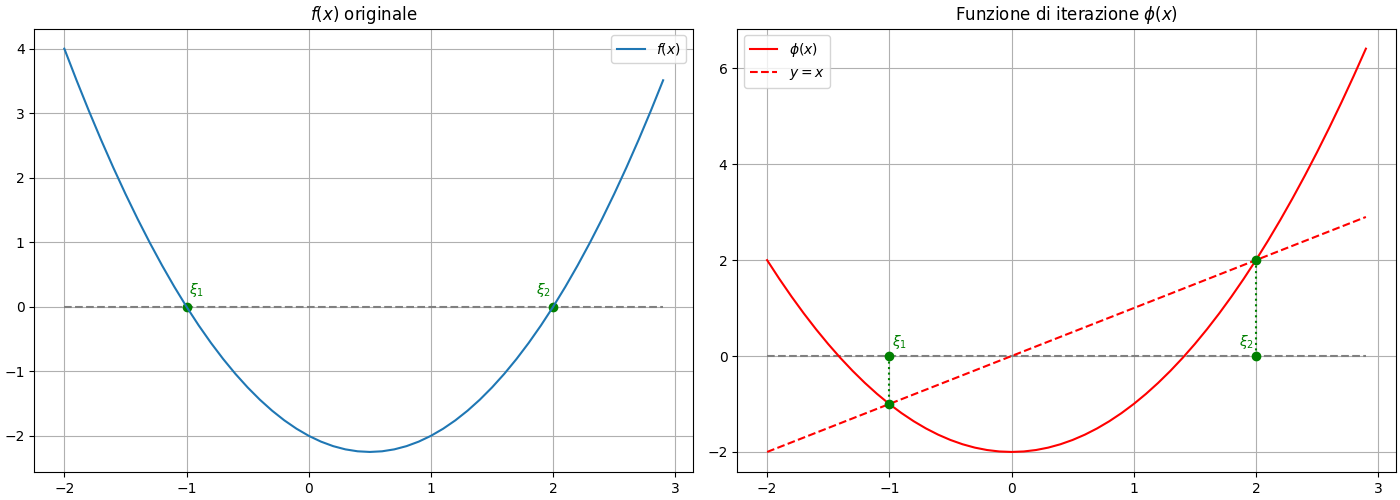
\includegraphics[width=\linewidth]{assets/image-006.png}
    \end{center}
\end{example}

Ma in cosa consiste dunque il metodo del punto unito? In sintesi, questo consente di trovare le radici di un'equazione riscrivendola prima in una forma equivalente, e poi recuperando le radici di questa forma equivalente:
\[ f(x) \eq 0 \quad \Longleftrightarrow \quad x \eq \phi(x) \]

Dunque, se $\xi$ è radice di $f$, allora questa sarà detta \textbf{punto unito} di $\phi$. In altre parole, trovare il punto unito di $\phi$ significa trovare l'ascissa di intersezione tra la retta $y \eq x$ e la curva data da $y \eq \phi(x)$. Una funzione $f$ può avere più di un punto unito, un solo punto o nessun punto unito.
\nwl
Questi metodi convergeranno se la successione delle approssimazioni $\{ x_n \eq \phi(x_{n - 1})\}_{n \geq 1}$ rispetta il seguente limite:
\[ \lim_{n \to \infty} |\xi - x_n| \eq 0 \quad \Longleftrightarrow \quad \lim_{n \to \infty} x_n \eq \xi \]

Se il metodo è convergente, allora una buona approssimazione di $\xi$ viene data dal valore $x_n$, rispettando dunque il seguente criterio:
\[ |x_n - x_{n - 1}| \leq \epsilon \]

\subsection{Convergenza del metodo del punto fisso}

La convergenza del metodo richiede che due condizioni siano soddisfatte: una necessaria e una sufficiente. Iniziamo a illustrare, in una maniera meglio formalizzata, la condizione necessaria:

\begin{theorem}{Condizione necessaria per la convergenza}
    Se la successione generata da:
    \[ \begin{cases}
        x_0 & \text{dato come input} \\
        x_n \eq \phi(x_{n - 1}) & \text{per } n \eq 1, \; 2, \; ...
    \end{cases} \]

    è convergente a un valore $\tau$ e $\phi$ è continua in $\tau$, allora $\tau$ è \textbf{punto unito} di $\phi$, cioè $\tau \eq \phi(\tau)$
\end{theorem}

Illustriamo ora un altro esempio, per meglio introdurre la condizione sufficiente di convergenza:

\begin{example}
    Consideriamo la funzione $f(x) \eq x^3 + 4x^2 - 10 \eq 0$: vogliamo verificare che, nell'intervallo $[1, \; 2]$ ci sia una singola radice, e vogliamo approssimare la radice tramite il metodo del punto unito.
    \nwl
    Possiamo verificare facilmente che la funzione ha una sola radice nell'intervallo specificato: infatti, non solo $f(1) \cdot f(2) < 0$, il che vuol dire che la funzione interseca l'asse $x$ almeno una volta, ma $f(x)$ è anche monotona crescente. Quest'ultima informazione ci viene data dalla derivata, che ha radici fuori dall'intervallo in cui siamo interessati. Dunque, la funzione è monotona crescente in $[1, \; 2]$, il che vuol dire che ha solo una radice nell'intervallo interessato.
    \nwl
    Ora passiamo al calcolare la funzione di iterazione. Possiamo trovarne almeno 5:
    \begin{itemize}
        \item [1)] tramite l'isolamento di $x^2$:
        \[ x^2 \eq \frac{10 - x^3}{4} \; \Longrightarrow \; x \eq \frac{\sqrt{10 - x^3}}{2} \eq \phi_1(x) \]

        \item [2)] tramite l'isolamento di $x^3$:
        \[ x^3 \eq 10 - 4x^2 \; \Longrightarrow \; x \eq \sqrt[3]{10 - 4x^2} \eq \phi_2(x) \]

        \item [3)] aggiungendo $-x$ a entrambi i membri:
        \[ x^3 + 4x^2 - 10 - x \eq -x \; \Longrightarrow \; x \eq -x^3 - 4x^2 + 10 + x \eq \phi_3(x) \]

        \item [4)] dividendo per $x$ e isolando $x^2$:
        \[ \frac{x^3 + 4x^2 - 10}{x} \eq 0 \; \Longrightarrow \; x \eq \left( \frac{10}{x} - 4x \right)^{\frac{1}{2}} \eq \phi_4(x) \]

        \item [5)] tramite il metodo di Newton:
        \[ x - \frac{f(x)}{f'(x)} \eq x \; \Longrightarrow \; x \eq x - \frac{x^3 + 4x^2 - 10}{3x^2 + 8x} \eq \phi_5(x) \]
    \end{itemize}

    Utilizziamo ora il metodo del punto fisso per produrre le approssimazioni della nostra radice $\xi$; per farlo, useremo il seguente algoritmo:
    \[ \begin{cases}
        x_0 \eq 1,5 & \\
        x_n \eq \phi(x_{n - 1}) & \text{per } n \eq 1, \; 2, \; ...
    \end{cases} \]

    Dopo 20 iterazioni per tutti i metodi, possiamo notare come solo alcune funzioni abbiano portato alla convergenza, benché tutte queste siano funzionalmente identiche:

    \begin{center}
        \resizebox{\linewidth}{!}{
            \renewcommand{\arraystretch}{1.3}
            \begin{tabular}{|c|c|c|c|c|c|}
                \hline
                \textbf{Iterazione} & $\mathbf{\phi_1(x)}$ & $\mathbf{\phi_2(x)}$ & $\mathbf{\phi_3(x)}$ & $\mathbf{\phi_4(x)}$ & $\mathbf{\phi_5(x)}$ \\
                \hline\hline 
                $1$ & $1.2869537676$ & $1.0000000000$ & $-0.875$ & $0.8164965809$ & $1.3733333333$ \\
                \hline 
                $2$ & $1.4025408035$ & $1.8171205928$ & $6.732421875$ & $2.9969088058$ & $1.3652620149$ \\
                \hline 
                $3$ & $1.3454583740$ & N/A & $-469.72001200$ & $1.0000000000$ & $1.3652300139$ \\
                \hline 
                $4$ & $1.3751702528$ & N/A & $102754555.19$ & $2.4494897428$ & $1.3652300134$ \\
                \hline 
                $5$ & $1.3600941928$ & N/A & $-1.0849338705 \cdot 10^{24}$ & $1.0000000000$ & $1.3652300134$ \\
                \hline 
                $6$ & $1.3678469676$ & N/A & $1.2770555914 \cdot 10^{72}$ & $2.4494897428$ & $1.3652300134$ \\
                \hline 
                $7$ & $1.3638870039$ & N/A & $-2.0827129086 \cdot 10^{216}$ & $1.0000000000$ & $1.3652300134$ \\
                \hline 
                $8$ & $1.3659167334$ & N/A & N/A & $2.4494897428$ & $1.3652300134$ \\
                \hline 
                $9$ & $1.3648782172$ & N/A & N/A & $1.0000000000$ & $1.3652300134$ \\
                \hline 
                $10$ & $1.3654100612$ & N/A & N/A & $2.4494897428$ & $1.3652300134$ \\
                \hline 
                $11$ & $1.3651378207$ & N/A & N/A & $1.0000000000$ & $1.3652300134$ \\
                \hline 
                $12$ & $1.3652772085$ & N/A & N/A & $2.4494897428$ & $1.3652300134$ \\
                \hline 
                $13$ & $1.3652058503$ & N/A & N/A & $1.0000000000$ & $1.3652300134$ \\
                \hline 
                $14$ & $1.3652423837$ & N/A & N/A & $2.4494897428$ & $1.3652300134$ \\
                \hline 
                $15$ & $1.3652236802$ & N/A & N/A & $1.0000000000$ & $1.3652300134$ \\
                \hline 
                $16$ & $1.3652332557$ & N/A & N/A & $2.4494897428$ & $1.3652300134$ \\
                \hline 
                $17$ & $1.3652283535$ & N/A & N/A & $1.0000000000$ & $1.3652300134$ \\
                \hline 
                $18$ & $1.3652308632$ & N/A & N/A & $2.4494897428$ & $1.3652300134$ \\
                \hline 
                $19$ & $1.3652295783$ & N/A & N/A & $1.0000000000$ & $1.3652300134$ \\
                \hline 
                $20$ & $1.3652302362$ & N/A & N/A & $2.4494897428$ & $1.3652300134$ \\
                \hline
            \end{tabular}
        }
    \end{center}

    Come possiamo notare, soltanto due funzioni riescono a convergere al valore della radice, mentre tutte le altre invece divergono (addirittura, $\phi_2(x)$ inizia a manifestare numeri complessi e $\phi_3(x)$ genera overflow dopo la 7$^{\text{a}}$ iterazione).
\end{example}

Con lo scorso esempio possiamo facilmente giungere alla conclusione che non tutte le funzioni di iterazione sono valide per essere usate con il metodo del punto unito. Serve dunque introdurre una nuova condizione, per meglio filtrare quali funzioni sono accettabili:

\begin{theorem}{Condizione sufficiente per la convergenza}
    Se una funzione d'iterazione $\phi$ è \textbf{derivabile} in un intorno $I \eq [a, \; b]$ e:
    \begin{itemize}
        \item con $\phi \; : \; I \; \longrightarrow \; I$, dove
        \[ a \leq \min_{x \in I} \phi(x) \leq \max_{x \in I} \phi(x) \leq b \]
        \item $\exists \; k \in (0, \; 1)$ tale che $|\phi'(x)| \leq k, \; \forall \; x \in I$;
    \end{itemize}

    allora:
    \begin{itemize}
        \item esiste un \textbf{unico punto unito} $\xi \in I$ di $\phi(\xi)$;
        \item la successione $x_n \eq \phi(x_{n - 1})$ è convergente a $\xi$ per ogni approssimazione iniziale $x_0 \in I$: in altre parole, $\phi$ deve essere una \textbf{contrazione}.
    \end{itemize}
\end{theorem}

Matematicamente, una contrazione è una funzione tale che, su tutto il dominio (nel nostro caso, su un intervallo specifico), per ogni $x$ del dominio allora la distanza tra due valori di $x$ qualsiasi (chiamati $x_1$ e $x_2$) è maggiore della distanza dell'immagine di questi:
\[ x_1 \leq f(x_1) \leq f(x_2) \leq x_2 \]

Circa la convergenza, possiamo fare un ulteriore appunto: dato un intervallo che rispetta le condizioni di convergenza, è possibile scegliere un sotto-intorno di $I$ all'interno del quale la successione di approssimazioni sarà sempre convergente per qualsiasi approssimazione iniziale scelta. La definizione formale è quella che segue:

\begin{theorem}{Seconda condizione sufficiente per la convergenza}
    Data una funzione di iterazione $\phi$, se questa è derivabile in $I \eq [a, \; b]$ e:
    \begin{itemize}
        \item $\phi(\xi) \eq \xi$, dove $\xi \in (a, \; b)$;
        \item $\exists \; k \in (0, \; 1)$ tale che $|\phi'(x)| \leq k, \; \forall x \in I$;
    \end{itemize}

    allora esiste un intorno di $\xi$ denotato con $\Delta$ (dove $\Delta \eq [\xi - \delta, \; \xi + \delta] \subseteq I$) tale che:
    \begin{itemize}
        \item $\xi$ è l'unico punto unito di $\phi(\xi)$ in $\Delta$;
        \item la successione $\{ x_n \eq \phi(x_{n - 1}) \}$, per $n \eq 1, \; 2, \; 3, \; ...$, è convergente a $\xi$ per ogni approssimazione iniziale $\x_0 \in \Delta$
    \end{itemize}
\end{theorem}

Possiamo anche utilizzare il metodo del punto fisso assieme al metodo delle tangenti:

\begin{theorem}{Applicazione del metodo del punto fisso al metodo delle tangenti}
    Se $I \eq [a, \; b]$ è un intervallo di separazione di una radice $\xi$ di $f$, e:
    \begin{itemize}
        \item $f, \; f', \; f''$ sono continue in $I$, tale che $f \in C^2 [a, \; b]$;
        \item $f'(x) \neq 0$ per $x \in [a, \; b]$;
    \end{itemize}

    allora esiste un intorno $J \subseteq I$ di $\xi$ tale che per $x_0 \in J$ la successione delle approssimazioni
    \[ \left\{ xn \eq x_{n - 1} - \frac{f(x_{n - 1})}{f'(x_{n - 1})} \right\} \]

    converge a $\xi$
\end{theorem}

Circa il metodo del punto fisso, nei scorsi teoremi circa la convergenza abbiamo usato più e più volte un intervallo $[0, \; 1)$, cercando di far sì che $|\phi'(x)|$ fosse all'interno di questo intervallo. Adesso ci concentreremo nel capire cosa succede se $\phi'(x)$ dovesse essere nell'intervallo $[0, \; 1)$ piuttosto che nell'intervallo $(-1, \; 0]$; come noteremo, questo avrà un effetto sull'errore del metodo. Per poter studiare questi comportamenti ci serviremo del teorema di Lagrange, il quale sostiene che, data una funzione continua in un intervallo $I \eq [a, \; b]$, allora esiste un punto $c \in I$ tale che
\[ f'(c) \eq \frac{f(b) - f(a)}{b - a} \]

Possiamo dunnque procedere a scrivere l'equazione dell'errore del metodo:
\begin{align*}
    e_n &\eq \xi - x_n \\
    &\eq \phi(\xi) - \phi(x_{n - 1}) \\
    &\eq \left(\phi(\xi) - \phi(x_{n - 1})\right) \cdot \frac{\xi - x_{n - 1}}{\xi - x_{n - 1}} \\
    &\eq \phi'(t_n) \cdot (\xi - x_{n - 1}) \\
    &\eq \phi'(t_n) \cdot e_{n - 1} \quad (\text{con } t_n \in [x_{n - 1}, \; \xi]) 
\end{align*}

Studiamo ora i due possibili casi, ovverosia se $\phi'(x) \in [0, \; 1)$ o se $\phi'(x) \in (-1, \; 0]$:
\begin{itemize}
    \item nel caso in cui $0 \leq \phi'(x) < 1$ per $x \in I$, la successione $\{x_n \eq \phi(x_{n - 1})\}$ (con $n \eq 1, \; 2, \; ...$) fosse monotona crescente (nel caso in cui $e_0 > 0$) o decrescente (se $e_0 < 0$), allora le approssimazioni all'interno della successione sarebbero per \textbf{difetto} (nel caso in cui $\xi > x_0$) o per \textbf{eccesso} (se $\xi < x_0$);
    \item nel caso in cui $-1 < \phi'(x) \leq 0$ per $x \in I$, la successione $\{x_n \eq \phi(x_{n - 1})\}$ (con $n \eq 1, \; 2, \; ...$) non fosse monotona, allora le approssimazioni all'interno della successione sarebbero \textbf{alternativamente per difetto e per eccesso}.
\end{itemize}